\section{}
\label{sec:p1}
%%%%%%%%%%%%%%%%%%%%%%%%%%%%%%%%%%%%%%%%%%%%%%%%%%%%%%%%%%%%%%%%%%%%%%
\paragraph{a)}
The '\textit{seismic.dat}' data contains seismic data on a regular grid $(75\times75)$, $L_D$, denoted as $\{d(\vect{x}) \ssep \vect{x}\in L_D\} \ssep d(\vect{x})\in \R$, and visually represented by the map in Figure \ref{fig:data}.
The seismic data has the likelihood model given by the equation
\begin{equation}
    [d_i\given\vect{l}] = \begin{cases}
                                0.02 + U_i, & l_i = 0 \Rightarrow \mathrm{sand} \\
                                0.08 + U_i, & l_i = 1 \Rightarrow \mathrm{shale}
                             \end{cases}
                            , i = 1, 2, ..., n,
    \label{eq:likelihood}
\end{equation}

where $U_i \overset{\mathrm{iid}}{\sim}\N\{0,0.06^2\}$. This means that we can rewrite Equation \ref{eq:likelihood} to 
\begin{equation}
    [d_i\given\vect{l}] = \begin{cases}
                                A_i\overset{\mathrm{iid}}{\sim}\N\{0.02,0.06^2\}, & l_i = 0 \Rightarrow \mathrm{sand} \\
                                B_i\overset{\mathrm{iid}}{\sim}\N\{0.08,0.06^2\}, & l_i = 1 \Rightarrow \mathrm{shale}
                             \end{cases}
                            , i = 1, 2, ..., n.
    \label{eq:likelihood2}
\end{equation}
The likelihood model $p(\vect{d}\given \vect{l})$ is then given by 
\begin{equation}
    \begin{array}{rcl}
        [\vect{d}\given\vect{l}] \sim p(\vect{d}\given\vect{l}) & = & \prod\limits_{i=1}^n p(d_i\given l_i) \\
        & = & (0.0072\pi)^{-n/2} \prod\limits_{i=1}^n l_i \exp\left\{\frac{(d_i - 0.08)^2}{0.0072} \right\} + (1-l_i) \exp\left\{\frac{(d_i - 0.02)^2}{0.0072} \right\} \\
         & = & (0.0072\pi)^{-n/2} \exp\left\{\frac{1}{0.0072} \left[\sum\limits_{i \st l_i = 0} (d_i - 0.02)^2 + \sum\limits_{i \st l_i = 1} (d_i - 0.08)^2\right]\right\} \, .
    \end{array}
    \label{eq:likelihood3}
\end{equation}

\begin{figure}
    \centering
    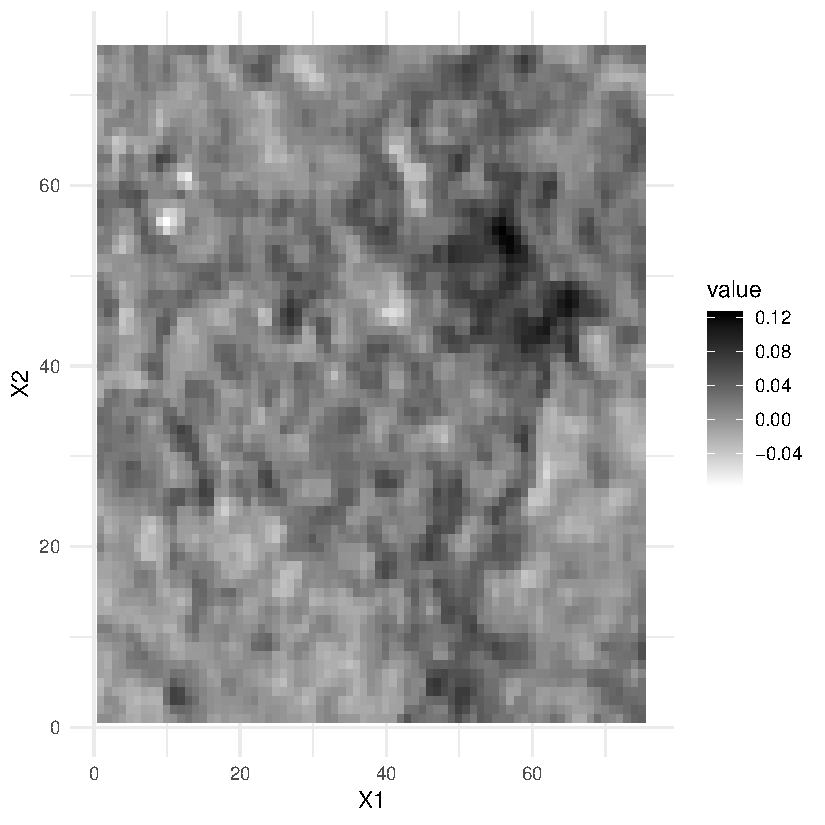
\includegraphics[scale=0.95]{figures/seismic_data.pdf}
    \caption{Map of the seismic data $d(\vect{x})$ on a grid $\matr{L_D}$}
    \label{fig:data}
\end{figure}
%%%%%%%%%%%%%%%%%%%%%%%%%%%%%%%%%%%%%%%%%%%%%%%%%%%%%%%%%%%%%%%%%%%%%%
\paragraph{b)}
With a uniform form prior $p(\vect{l}) = const$, the posterior becomes
%
\begin{equation}
\label{eq:b_post}
\begin{split}
    p(\vect{l} \given \vect{d}) &= \frac{p(\vect{d} \given \vect{l}) p(\vect{l})}{\sum_{\vect{l'} \in L_D} p(\vect{d} \given \vect{l}) p(\vect{l})} \\
    &= \frac{p(\vect{d} \given \vect{l})}{\sum_{\vect{l'} \in L_D} p(\vect{d} \given \vect{l}))} \\
    &= \frac{\exp\left\{\frac{1}{0.0072} \sum_{i=1}^n \left[(1-l_i)(d_i - 0.02)^2 + l_i(d_i - 0.08)^2\right]\right\}}{\sum_{\vect{l'} \in L_D} \exp\left\{\frac{1}{0.0072} \sum_{i=1}^n \left[(1-l_i')(d_i - 0.02)^2 + l_i'(d_i - 0.08)^2\right]\right\}} \, .
\end{split}
\end{equation}
%

%%%%%%%%%%%%%%%%%%%%%%%%%%%%%%%%%%%%%%%%%%%%%%%%%%%%%%%%%%%%%%%%%%%%%%
\paragraph{c)}


%%%%%%%%%%%%%%%%%%%%%%%%%%%%%%%%%%%%%%%%%%%%%%%%%%%%%%%%%%%%%%%%%%%%%%
\paragraph{d)}

